\documentclass[a4paper,xelatex,english]{bxjsarticle}
\usepackage{tikz}%
\usetikzlibrary{arrows.meta,bending,calc,shapes,positioning,shapes.callouts}
\usepackage{ascmac}
\usepackage{fancybox}
\usepackage{amsmath,amssymb}
\usepackage{algorithm}
\usepackage{algpseudocode}
\usepackage{paralist}
\usepackage{cases}
\usepackage{url}
\usepackage[unicode,pdftitle={Implementation Notes for entropy estimation based on NIST SP 800-90B non-IID track},setpagesize=false]{hyperref}
\usepackage[open,openlevel=4]{bookmark}
\newcommand\mib[1]{\boldsymbol{#1}}

\usepackage{xcolor}
\usepackage{fancyhdr}
\usepackage[explicit]{titlesec}
\usepackage{xspace}

\usepackage[many]{tcolorbox}
%%%%%%%%%%%%%%%%%%%%%%%%%%%%%%%%%%%%%%%%%%%%%%%%%%%%%%%%%%%%%%%%%%%%%%%%%%%%%%%%
%%%
%%%
%%%
%%%%%%%%%%%%%%%%%%%%%%%%%%%%%%%%%%%%%%%%%%%%%%%%%%%%%%%%%%%%%%%%%%%%%%%%%%%%%%%%
\definecolor{mydarkblue}{RGB}{0,163,243}
\definecolor{mylightblue}{RGB}{191,233,251}
\definecolor{mediumtealblue}{rgb}{0.0, 0.33, 0.71}
%%%%%%%%%%%%%%%%%%%%%%%%%%%%%%%%%%%%%%%%%%%%%%%%%%%%%%%%%%%%%%%%%%%%%%%%%%%%%%%%
%%%
%%%
%%%
%%%%%%%%%%%%%%%%%%%%%%%%%%%%%%%%%%%%%%%%%%%%%%%%%%%%%%%%%%%%%%%%%%%%%%%%%%%%%%%%
%\def\chpcolor{blue!45}
\def\chpcolor{mydarkblue}
%\def\chpcolortxt{blue!60}
\def\chpcolortxt{mydarkblue}
\def\sectionfont{\sffamily\LARGE}

%%%%%%%%%%%%%%%%%%%%%%%%%%%%%%%%%%%%%%%%%%%%%%%%%%%%%%%%%%%%%%%%%%%%%%%%%%%%%%%
%%%%%%
%%%%%% 4-th level
%%%%%%
%%%%%%%%%%%%%%%%%%%%%%%%%%%%%%%%%%%%%%%%%%%%%%%%%%%%%%%%%%%%%%%%%%%%%%%%%%%%%%%
\setcounter{secnumdepth}{4}

\setcounter{tocdepth}{4}

%%%%%%%%%%%%%%%%%%%%%%%%%%%%%%%%%%%%%%%%%%%%%%%%%%%%%%%%%%%%%%%%%%%%%%%%%%%%%%%
%%%%%%
%%%%%%
%%%%%%
%%%%%%%%%%%%%%%%%%%%%%%%%%%%%%%%%%%%%%%%%%%%%%%%%%%%%%%%%%%%%%%%%%%%%%%%%%%%%%%
\makeatletter
%Section:
\def\@sectionstrut{\vrule\@width\z@\@height12.5\p@}
\def\@makesectionhead#1{%
  {\par\vspace{20pt}%
   \parindent 0pt\raggedleft\sectionfont
   \colorbox{\chpcolor}{%
     \parbox[t]{90pt}{\color{white}\@sectionstrut\@depth4.5\p@\hfill
       \ifnum\c@secnumdepth>\z@\thesection\fi}%
   }%
   \begin{minipage}[t]{\dimexpr\textwidth-90pt-2\fboxsep\relax}
   \color{\chpcolortxt}\@sectionstrut\hspace{5pt}#1
   \end{minipage}\par
   \vspace{10pt}%
  }
}
\def\section{\@afterindentfalse\secdef\@section\@ssection}
\def\@section[#1]#2{%
  \ifnum\c@secnumdepth>\m@ne
    \refstepcounter{section}%
    \addcontentsline{toc}{section}{\protect\numberline{\thesection}#1}%
  \else
    \phantomsection
    \addcontentsline{toc}{section}{#1}%
  \fi
  \sectionmark{#1}%
  \if@twocolumn
    \@topnewpage[\@makesectionhead{#2}]%
  \else
    \@makesectionhead{#2}\@afterheading
  \fi
}
\def\@ssection#1{%
  \if@twocolumn
    \@topnewpage[\@makesectionhead{#1}]%
  \else
    \@makesectionhead{#1}\@afterheading
  \fi
}
\makeatother
%%%%%%%%%%%%%%%%%%%%%%%%%%%%%%%%%%%%%%%%%%%%%%%%%%%%%%%%%%%%%%%%%%%%%%%%%%%%%%%%
%%%
%%%
%%%
%%%%%%%%%%%%%%%%%%%%%%%%%%%%%%%%%%%%%%%%%%%%%%%%%%%%%%%%%%%%%%%%%%%%%%%%%%%%%%%%
\newsavebox\mybox
\newlength\secnumwd

%\definecolor{mydarkblue}{RGB}{0,163,243}
%\definecolor{mylightblue}{RGB}{191,233,251}

\titleformat{\section}
  {\normalfont\Large\sffamily\color{mydarkblue}}
  {}
  {-5em}
  {%
    \savebox\mybox{\normalfont\Large\sffamily\color{mydarkblue}\bfseries\thesection}%
    \settowidth\secnumwd{\usebox\mybox}%    
    \parbox[t]{\secnumwd}{{\bfseries\thesection}}\hspace{1em}%
    \parbox[t]{\dimexpr\textwidth+5em-\secnumwd-1em\relax}{#1}%
  }
  [\vskip-1.75ex\hskip-5em{\color{gray!60}\titlerule[2pt]}]
\titleformat{name=\section,numberless}
  {\normalfont\Large\sffamily\color{mydarkblue}}
  {}
  {-5em}
  {#1}
  [\vskip-1.75ex\hskip-5em{\color{gray!60}\titlerule[2pt]}]

\newcommand\FrameBoxL[1]{%
  \fcolorbox{mylightblue}{mydarkblue}{\makebox[3cm][l]{\textcolor{white}{\bfseries#1}}}%
}
\newcommand\FrameBoxR[1]{%
  \fcolorbox{mylightblue}{mydarkblue}{\makebox[3cm][r]{\textcolor{white}{\bfseries#1}}}%
}

\pagestyle{fancy}
\fancyheadoffset[EL]{\dimexpr1in+\evensidemargin+\hoffset\relax}
\fancyheadoffset[OR]{\dimexpr\paperwidth-\oddsidemargin-1in-\textwidth-\hoffset\relax}
\fancyhf{}
\renewcommand\headrulewidth{0pt}
\fancyhead[OR]{\FrameBoxL{\thepage}}
\fancyhead[EL]{\FrameBoxR{\thepage}}
%%%%%%%%%%%%%%%%%%%%%%%%%%%%%%%%%%%%%%%%%%%%%%%%%%%%%%%%%%%%%%%%%%%%%%%%%%%%%%%%
%%%
%%% argmax
%%%
%%%%%%%%%%%%%%%%%%%%%%%%%%%%%%%%%%%%%%%%%%%%%%%%%%%%%%%%%%%%%%%%%%%%%%%%%%%%%%%%
\newcommand{\argmax}{\mathop{\textrm{arg~max}}\limits}
%%%%%%%%%%%%%%%%%%%%%%%%%%%%%%%%%%%%%%%%%%%%%%%%%%%%%%%%%%%%%%%%%%%%%%%%%%%%%%%%
%%%
%%% vertical equal
%%%
%%%%%%%%%%%%%%%%%%%%%%%%%%%%%%%%%%%%%%%%%%%%%%%%%%%%%%%%%%%%%%%%%%%%%%%%%%%%%%%%
\newcommand\rotateequal[1]{%
  \ifmmode
    \underset{#1}{\rotatebox{90}{$=$}}%
  \fi
}
%%%%%%%%%%%%%%%%%%%%%%%%%%%%%%%%%%%%%%%%%%%%%%%%%%%%%%%%%%%%%%%%%%%%%%%%%%%%%%%%
%%%
%%%
%%%
%%%%%%%%%%%%%%%%%%%%%%%%%%%%%%%%%%%%%%%%%%%%%%%%%%%%%%%%%%%%%%%%%%%%%%%%%%%%%%%%
\algnewcommand{\algorithmicgoto}{\textbf{go to}}%
\algnewcommand{\Goto}{\algorithmicgoto\xspace}%
\algnewcommand{\Label}{\State\unskip}
%%%%%%%%%%%%%%%%%%%%%%%%%%%%%%%%%%%%%%%%%%%%%%%%%%%%%%%%%%%%%%%%%%%%%%%%%%%%%%%%
%%%
%%%
%%%
%%%%%%%%%%%%%%%%%%%%%%%%%%%%%%%%%%%%%%%%%%%%%%%%%%%%%%%%%%%%%%%%%%%%%%%%%%%%%%%%
\definecolor{myblue}{RGB}{0,163,243}

\newtcolorbox[auto counter,number within=section]{mytheorem}[1][]{
  enhanced jigsaw,colback=white,colframe=myblue,coltitle=myblue,
  fonttitle=\bfseries\sffamily,
  sharp corners,
  detach title,
  leftrule=22mm,
  underlay unbroken and first={\node[below,text=white,font=\sffamily\bfseries,align=center]
    at ([xshift=-11mm,yshift=-1mm]interior.north west) {THEOREM\\\thetcbcounter};},
  breakable,pad at break=1mm,
  #1,
  code={\ifdefempty{\tcbtitletext}{}{\tcbset{before upper={\tcbtitle\par\medskip}}}},
}

%%%\usepackage{titlesec}
%%%%%%\usepackage{lipsum}
%%%\usepackage{tikz}\usetikzlibrary{shapes.misc}
%%%\newcommand\titlebar{%
%%%\tikz[baseline,trim left=3.1cm,trim right=3cm] {
%%%    \fill [cyan!25] (2.5cm,-1ex) rectangle (\textwidth+3.1cm,2.5ex);
%%%    \node [
%%%        fill=cyan!60!white,
%%%        anchor= base east,
%%%        %rounded rectangle,
%%%        rectangle,
%%%        minimum height=3.5ex] at (3cm,0) {
%%%        \textbf{\thesection.}
%%%    };
%%%}%
%%%}
%%%\titleformat{\section}{\large}{\titlebar}{0.1cm}{}
%%%\renewcommand*{\thesection}{\arabic{section}}

%%%\usepackage{xcolor}
%%%
%%%\setcounter{section}{1} % just to emulate a chapter has started
%%%
%%%\renewcommand*{\othersectionlevelsformat}[1]{%
%%%  \makebox[0pt][r]{%
%%%    \fcolorbox{cyan!60!white}{cyan!60!white}{\color{white}\csname the#1\endcsname}%
%%%    \enskip
%%%  }
%%%}


\renewcommand{\figurename}{Figure }
\renewcommand{\tablename}{Table }
\renewcommand{\refname}{References}
\renewcommand*{\thesection}{\arabic{section}}
\title{Implementation Notes for entropy estimation based on NIST SP 800-90B non-IID track}
\date{\today}
\begin{document}
\maketitle
%%%%%%%%%%%%%%%%%%%%%%%%%%%%%%%%%%%%%%%%%%%%%%%%%%%%%%%%%%%%%%%%%%%
%%%%%
%%%%%
%%%%%
%%%%%%%%%%%%%%%%%%%%%%%%%%%%%%%%%%%%%%%%%%%%%%%%%%%%%%%%%%%%%%%%%%%
\section{Implementation notes for numerical computation of entropy estimates}
\renewcommand{\arraystretch}{1.4}
%%%%%%%%%%%%%%%%%%%%%%%%%%%%%%%%%%%%%%%%%%%%%%%%%%%%%%%%%%%%%%%%%%%
%%%%%
%%%%%
%%%%%
%%%%%%%%%%%%%%%%%%%%%%%%%%%%%%%%%%%%%%%%%%%%%%%%%%%%%%%%%%%%%%%%%%%
\subsection{Notes for the Markov estimate}
In this section, we follow the convention using a column vector of probabilities $\mib{P}$ and a left stochastic matrix $\mib{T}$.
\begin{align}
\mib{P} 
\equiv 
& 
\begin{bmatrix}
p_{0} \\
p_{1} \\
\end{bmatrix} 
\\
%%%%%
%%%%%
%%%%%
\mib{T} 
\equiv 
& 
\begin{bmatrix}
t_{0,0} & t_{0,1} \\
t_{1,0} & t_{1,1}
\end{bmatrix}
\end{align}
Note here that 6.3.3 of NIST SP 800-90B\cite{SP80090B} uses the convention of a row vector of probabilities and a right stochastic matrix.  So the transition matrix components $t_{i,j}$ in this section will be interpreted as $t_{j,i}$ in 6.3.3 of NIST SP 800-90B\cite{SP80090B}.


Considering a sequence of binary-valued samples of length $\lambda$, there are following four possible combinations of the first sample value and the last sample value:\begin{enumerate}[a)]
	\item 0 $\to$ 0
	\item 0 $\to$ 1
	\item 1 $\to$ 0
	\item 1 $\to$ 1
\end{enumerate}

For each combination, the probability of occurrence of the most likely sequence is expressed by the following equation, by using the parameters $\mu$ and $\nu$:
\begin{enumerate}[a)]
	%%%%%
	%%%%% a)
	%%%%%
	\item 
	\begin{align}
		f_{a}(\mib{T}, \mu, \nu) & \equiv p_{0} t_{00}^{\nu} t_{11}^{\lambda - 1 - 2\mu - \nu} t_{01}^{\mu} t_{10}^{\mu} 
	\end{align}
	\begin{align}
	\begin{cases}
		0 \leq 2 \mu < \lambda - 1 & \\
		0 \leq \nu \leq \lambda - 1 & \\
		0 \leq \lambda - 1 - 2\mu - \nu \leq \lambda - 1
	\end{cases}
	\label{eq:fa}
	\end{align}
	%%%%%
	%%%%% b)
	%%%%%
	\item 
	\begin{align}
		f_{b}(\mib{T}, \mu, \nu) & \equiv p_{0} t_{00}^{\nu} t_{11}^{\lambda - 2 - 2\mu - \nu} t_{01}^{\mu} t_{10}^{\mu + 1} 
	\end{align}
	\begin{align}
	\begin{cases}
		0 \leq 2 \mu < \lambda - 1 & \\
		0 \leq \nu < \lambda - 1 & \\
		0 \leq \lambda - 2 - 2\mu - \nu \leq \lambda - 2
	\end{cases}
	\label{eq:fb}
	\end{align}
	%%%%%
	%%%%% c)
	%%%%%
	\item 
	\begin{align}
		f_{c}(\mib{T}, \mu, \nu) & \equiv p_{1} t_{00}^{\nu} t_{11}^{\lambda - 2 - 2\mu - \nu} t_{01}^{\mu + 1} t_{10}^{\mu} 
	\end{align}
	\begin{align}
	\begin{cases}
		0 \leq 2 \mu < \lambda - 1 & \\
		0 \leq \nu < \lambda - 1 & \\
		0 \leq \lambda - 2 - 2\mu - \nu \leq \lambda - 2
	\end{cases}
	\label{eq:fc}
	\end{align}
	%%%%%
	%%%%% d)
	%%%%%
	\item 
	\begin{align}
		f_{d}(\mib{T}, \mu, \nu) & \equiv p_{1} t_{00}^{\nu} t_{11}^{\lambda - 1 - 2\mu - \nu} t_{01}^{\mu} t_{10}^{\mu} 
	\end{align}
	\begin{align}
	\begin{cases}
		0 \leq 2 \mu < \lambda - 1 & \\
		0 \leq \nu \leq \lambda - 1 & \\
		0 \leq \lambda - 1 - 2\mu - \nu \leq \lambda - 1
	\end{cases}
	\label{eq:fd}
	\end{align}
\end{enumerate}

If we denote $\kappa$ as the exponent of $t_{11}$, then the possible values of $\mu, \nu$, and $\kappa$ are expressed as integer coordinates in the approximately triangular region (to be precise, truncated triangle) shown in Figure \ref{fig:parameterplane}.
\begin{figure}[htbp]
\centering

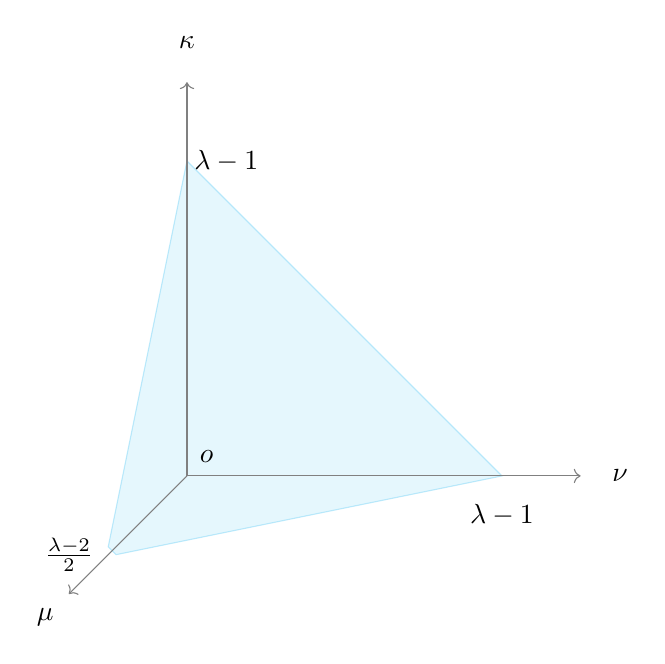
\begin{tikzpicture}
	\filldraw[fill=cyan!20, draw=cyan!50, opacity=0.5] (-0.9, -1) -- (4, 0) -- (0, 4) -- (-1, -0.9) -- (-0.9, -1);
	\draw[->,gray] ( 0, 0) -- (5, 0);
	\draw[->,gray] ( 0, 0) -- (0, 5);
	\draw[->,gray] ( 0, 0) -- (-1.5, -1.5);
	\draw (5.5, 0) node {$\nu$} ;
	\draw (-1.8, -1.8) node {$\mu$} ;
	\draw (0, 5.5) node {$\kappa$} ;
	%%%%%
	\draw ( 0.25, 0.25) node {$o$} ;
	\draw ( 4, -0.5) node {$\lambda - 1$} ;
	\draw ( 0.5,  4) node {$\lambda - 1$} ;
	\draw (-1.5, -1) node {$\frac{\lambda - 2}{2}$} ;
\end{tikzpicture}

\caption{Parameter plane of the exponents $\kappa$, $\mu$, $\nu$}
\label{fig:parameterplane}
\end{figure}

In order to calculate the extreme values of $f_{a}, f_{b}, f_{c}$, and $f_{d}$, assuming that $\mu$, and $\nu$ are continuous variables, we first consider the partial derivatives of $f_{a}(\mib{T}, \mu, \nu)$ with respect to $\mu$, and $\nu$.

\begin{align}
	\frac{\partial }{\partial \mu} f_{a}(\mib{T}, \mu, \nu) 
	&= 
	(-2 \ln t_{11} + \ln t_{01} + \ln t_{10}) f_{a}(\mib{T}, \mu, \nu) 
	\nonumber \\
	&= 
	\ln \frac{t_{01} t_{10}}{t_{11}^{2}} 
	f_{a}(\mib{T}, \mu, \nu) 
	\label{eq:nondiagonalproduct}
	\\
	%%%%%
	\frac{\partial }{\partial \nu} f_{a}(\mib{T}, \mu, \nu) 
	&= 
	(\ln t_{00} - \ln t_{11}) f_{a}(\mib{T}, \mu, \nu) 
	\nonumber \\
	&= 
	\ln \frac{t_{00}}{t_{11}} 
	f_{a}(\mib{T}, \mu, \nu) 
	\label{eq:diagonal}
\end{align}

%The partial derivatives of $f_{b}, f_{c}$, and $f_{d}$ with respect to $\mu$ and $\nu$ are obtained by taking permutation of $a$ with respecto to $b$, $c$, and $d$ in eq. (\ref{eq:nondiagonalproduct}) and eq.(\ref{eq:diagonal}), respectively.

Taking into accout eqs. (\ref{eq:nondiagonalproduct}) and (\ref{eq:diagonal}), and the property that the value $f_{a}(\mib{T}, \mu, \nu)$ is non-negative, 
a rough phase diagram will be obtained as shown in Figure \ref{fig:phasediagram}, by taking the horizontal axis as $\ln \frac{t_{00}}{t_{11}}$, and the vertical axis $\tfrac{1}{2}\ln \frac{t_{01} t_{10}}{t_{11}^{2}}$.

\begin{figure}[htbp]
\centering

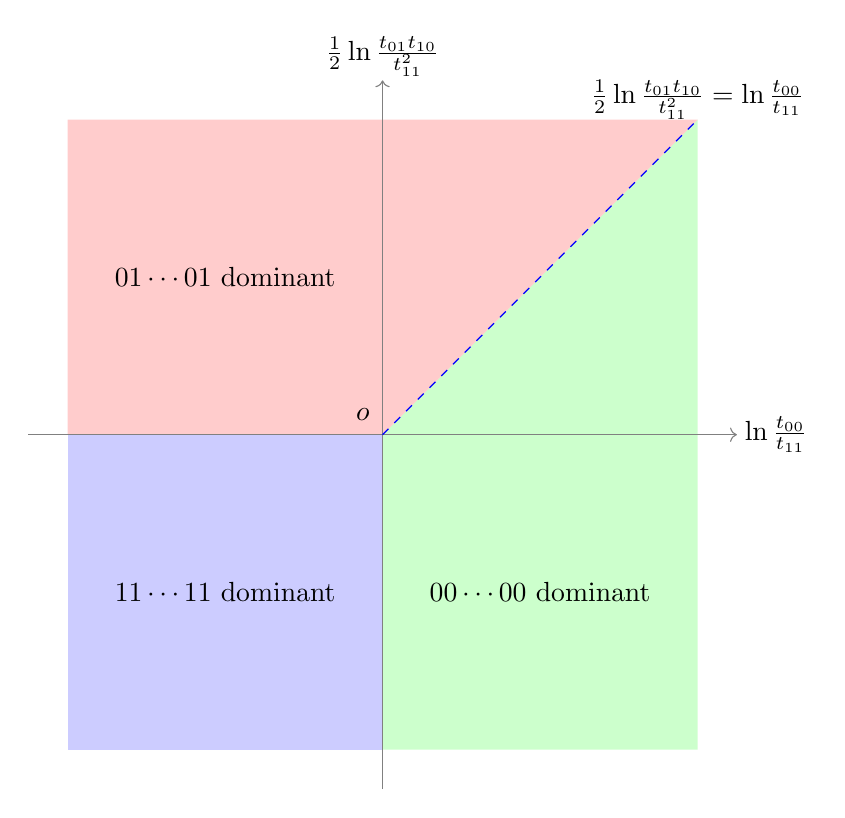
\begin{tikzpicture}
	\fill[green!20] (0, 0) -- (4,4) -- (4, -4) -- (0, -4);
	\fill[red!20] (0, 0) -- (4, 4) -- (-4,4) -- (-4, 0);
	\fill[blue!20] (0, 0) -- (0, -4) -- (-4,-4) -- (-4, 0);
	\draw[->,gray] (-4.5, 0) -- (4.5, 0);
	\draw[->,gray] ( 0,-4.5) -- (0, 4.5);
	\draw (-0.25, 0.25) node {$o$} ;
	\draw (5, 0) node {$\ln \frac{t_{00}}{t_{11}}$} ;
	\draw (0, 4.8) node {$\tfrac{1}{2} \ln \frac{t_{01} t_{10}}{t_{11}^{2}}$} ;
	\draw[blue,dashed] (0, 0) -- (4, 4);
	\draw (4, 4.25) node {$\tfrac{1}{2} \ln \frac{t_{01} t_{10}}{t_{11}^{2}} = \ln \frac{t_{00}}{t_{11}}$} ;
	%%%%%
	\draw ( 2, -2) node {$00 \cdots 00$ dominant} ;
	\draw (-2,  2) node {$01 \cdots 01$ dominant} ;
	\draw (-2, -2) node {$11 \cdots 11$ dominant} ;
\end{tikzpicture}

\caption{Phase diagram of most likely sequence based on $f_{a}(\mib{T}, \mu, \nu)$ with respect to components of transition probability matrix $\mib{T}$}
\label{fig:phasediagram}
\end{figure}

First, if we consider the third quadrant, for example, the conditional probability $t_{11}$ is greater than or equal to $t_{00}$ and $\sqrt{t_{01}t_{10}}$, then the sequence $11 \cdots 11$ will be dominant.

Next, for the other quadrants, let us consider whether $00 \cdots 00$ or $01 \cdots 01$ is the dominant sequence. 
In particular, for the first quadrant, since right hand sides of eqs. (\ref{eq:nondiagonalproduct}) and (\ref{eq:diagonal}) are positive, let us examine whether $00 \cdots 00$ or $0101 \cdots 0101$ is the dominant sequence. 
Since at least $11 \cdots 11$ is not a dominant sequence, we can limit the discussion with $\kappa =$ 0, 1, the parameter region of possible values of $\mu$ and $\nu$ is restricted to the line segment in Figure \ref{fig:parameterplane}. 
The delta of $f_{a}$ is then expressed by the following equation:
\begin{align}
\Delta f_{a} 
&= 
\left( 
\frac{\partial f_{a}}{\partial \mu} 
+ 
\frac{\partial f_{a}}{\partial \nu} 
\frac{{\mathrm d} \nu}{{\mathrm d} \mu}
\right) 
\Delta \mu 
\nonumber 
\\
&= 
\left(
\ln \frac{t_{01}t_{10}}{t_{00}^{2}}
\right)
\Delta \mu
\end{align}

From this equation, if RHS of eq. (\ref{expression:separationline}) is positive, $f_{a}$ increases with respect to $\mu$ and $01 \cdots 01$ becomes the dominant sequence, and conversely, if RHS of eq. (\ref{expression:separationline}) is negative, $00 \cdots 00$ becomes the dominant sequence.

\begin{align}
	\ln \frac{t_{01}t_{10}}{t_{00}^{2}} 
	&= 
	\ln \frac{t_{01}t_{10}}{t_{11}^{2}} - 2 \ln \frac{t_{00}}{t_{11}}
	\label{expression:separationline}
\end{align}
A diagonal straight line is shown in Figure \ref{fig:phasediagram} where the RHS of eq. (\ref{expression:separationline}) is zero.  
In other words, in the region above this line, $01 \cdots 01$ is the dominant sequence, and $00 \cdots 00$ is the dominant sequence in the region below the line. 


From the above, we have to consider the following three dominant sequences:
\begin{enumerate}[i)]
	\item $00 \cdots 00$ dominant 
	\item $01 \cdots 01$ dominant 
	\item $11 \cdots 11$ dominant 
\end{enumerate}
For each of $f_a, f_b, f_c$, and $f_d$, considering combination with above three dominant sequence, 
the following expressions give maximum value with respect to $\mu$ and $\nu$:

\begin{enumerate}[{a)}-i)]
	\item $00 \cdots 00$ dominant 
	\begin{align}
	\max_{\mu, \nu}(f_{a}(\mib{T}, \mu, \nu)) = p_{0} t_{00}^{\lambda - 1}
	\end{align}
	\item $01 \cdots 01$ dominant 
	\begin{align}
	\max_{\mu, \nu}(f_{a}(\mib{T}, \mu, \nu)) = & p_{0} t_{00} t_{01}^{(\lambda - 2) / 2} t_{10}^{(\lambda - 2) / 2}, {\textrm{or}} \\
	\max_{\mu, \nu}(f_{a}(\mib{T}, \mu, \nu)) = & p_{0} t_{11} t_{01}^{(\lambda - 2) / 2} t_{10}^{(\lambda - 2) / 2}
	\end{align}
	\item $11 \cdots 11$ dominant 
	\begin{align}
	\max_{\mu, \nu}(f_{a}(\mib{T}, \mu, \nu)) = p_{0} t_{11}^{\lambda - 3} t_{01} t_{10} \label{expression:neg1}
	\end{align}
\end{enumerate}

\begin{enumerate}[{b)}-i)]
	\item $00 \cdots 00$ dominant 
	\begin{align}
	\max_{\mu, \nu}(f_{b}(\mib{T}, \mu, \nu)) = p_{0} t_{00}^{\lambda - 2} t_{10}
	 \label{expression:nonneg1}
	\end{align}
	\item $01 \cdots 01$ dominant 
	\begin{align}
	\max_{\mu, \nu}(f_{b}(\mib{T}, \mu, \nu)) = p_{0} t_{01}^{(\lambda - 2) / 2} t_{10}^{\lambda / 2}
	\end{align}
	\item $11 \cdots 11$ dominant 
	\begin{align}
	\max_{\mu, \nu}(f_{b}(\mib{T}, \mu, \nu)) = p_{0} t_{11}^{\lambda - 2} t_{10} \label{expression:neg2}
	\end{align}
\end{enumerate}

\begin{enumerate}[{c)}-i)]
	\item $00 \cdots 00$ dominant 
	\begin{align}
	\max_{\mu, \nu}(f_{c}(\mib{T}, \mu, \nu)) = p_{1} t_{00}^{\lambda - 2} t_{01} \label{expression:neg3}
	\end{align}
	\item $01 \cdots 01$ dominant 
	\begin{align}
	\max_{\mu, \nu}(f_{c}(\mib{T}, \mu, \nu)) = p_{1} t_{01}^{\lambda / 2} t_{10}^{(\lambda - 2) / 2}
	\end{align}
	\item $11 \cdots 11$ dominant 
	\begin{align}
	\max_{\mu, \nu}(f_{c}(\mib{T}, \mu, \nu)) = p_{1} t_{11}^{\lambda - 2} t_{01}
	\end{align}
\end{enumerate}

\begin{enumerate}[{d)}-i)]
	\item $00 \cdots 00$ dominant 
	\begin{align}
	\max_{\mu, \nu}(f_{d}(\mib{T}, \mu, \nu)) = p_{1} t_{00}^{\lambda - 3} t_{01} t_{10} \label{expression:neg4}
	\end{align}
	\item $01 \cdots 01$ dominant 
	\begin{align}
	\max_{\mu, \nu}(f_{d}(\mib{T}, \mu, \nu)) = & p_{1} t_{00} t_{01}^{(\lambda - 2) / 2} t_{10}^{(\lambda - 2) / 2}, {\textrm{or}} \\
	\max_{\mu, \nu}(f_{d}(\mib{T}, \mu, \nu)) = & p_{1} t_{11} t_{01}^{(\lambda - 2) / 2} t_{10}^{(\lambda - 2) / 2}
	\end{align}
	\item $11 \cdots 11$ dominant 
	\begin{align}
	\max_{\mu, \nu}(f_{d}(\mib{T}, \mu, \nu)) = p_{1} t_{11}^{\lambda - 1}
	\end{align}
\end{enumerate}
Note here that the property that $\lambda$ is even is applied in above calculation.
Also note that all bounary conditions are considered in the above calculation, combination of first sample values and last sample values.


From the above, we have to compare 14 expressions listed in Table \ref{tab:ListProbabilitiesMostLikelySequences}.

\begin{table}[htbp]
\caption{Probabilities of the most or second most likely sequences of length $\lambda$}
\label{tab:ListProbabilitiesMostLikelySequences}
\begin{center}

\begin{tabular}{|r|l|c|c|l|}
\hline
No. & Sequence & Probability & $-\log_{2} ({\textrm{Probability}}) / \lambda$ & Notes\\
\hline 
1 & $0000 \cdots 0000$ & $p_{0} \times t_{00}^{\lambda - 1}$ & $-\left[ \frac{\lambda - 1}{\lambda} \log_{2} t_{00} + \frac{1}{\lambda} \log_{2} p_{0} \right]$ & $^{\textrm{\,a}}$, $^{\textrm{\,b}}$\\
\hline
2 & $0101 \cdots 0101001010 \cdots 1010$ & $p_{0} \times t_{00} \times t_{01}^{(\lambda - 2) / 2} \times t_{10}^{(\lambda - 2) / 2}$ & $-\left[ \frac{\lambda - 2}{2\lambda} \log_{2} \left( t_{01} t_{10} \right) + \frac{1}{\lambda} \log_{2} \left( p_{0} \times t_{00} \right) \right]$ & \quad $^{\textrm{\,b}}$ \\
\hline
3 & $0101 \cdots 0101101010 \cdots 1010$ & $p_{0} \times t_{11} \times t_{01}^{(\lambda - 2) / 2} \times t_{10}^{(\lambda - 2) / 2}$ & $-\left[ \frac{\lambda - 2}{2\lambda} \log_{2} \left( t_{01} t_{10} \right) + \frac{1}{\lambda} \log_{2} \left( p_{0} \times t_{11} \right) \right]$ &  \\
\hline 
4 & $0111 \cdots 1110$ & $p_{0} \times t_{11}^{\lambda - 3} \times t_{01} \times t_{10}$ & $-\left[ \frac{\lambda - 3}{\lambda} \log_{2} t_{11}+ \frac{1}{\lambda} \log_{2} \left( p_{0} \times t_{01} \times t_{10} \right)\right]$ &  \\
\hline 
5 & $0000 \cdots 0001$ & $p_{0} \times t_{00}^{\lambda - 2} \times t_{10}$ & $-\left[ \frac{\lambda - 2}{\lambda} \log_{2} t_{00}+ \frac{1}{\lambda} \log_{2} \left( p_{0} \times t_{10} \right)\right]$ &  \\
\hline 
6 & $0101 \cdots 0101$ & $p_{0} \times t_{01}^{(\lambda - 2) / 2} \times t_{10}^{\lambda / 2}$ & $-\left[ \frac{\lambda - 2}{2\lambda} \log_{2} \left( t_{01} t_{10} \right) + \frac{1}{\lambda} \log_{2} \left( p_{0} \times t_{10} \right) \right]$ & $^{\textrm{\,a}}$, $^{\textrm{\,b}}$ \\
\hline 
7 & $0111 \cdots 1111$ & $p_{0} \times t_{11}^{\lambda - 2} \times t_{10}$ & $-\left[ \frac{\lambda - 2}{\lambda} \log_{2} t_{11}+ \frac{1}{\lambda} \log_{2} \left( p_{0} \times t_{10} \right)\right]$ & $^{\textrm{\,a}}$, \quad $^{\textrm{\,c}}$\\
\hline 
8 & $1000 \cdots 0000$ & $p_{1} \times t_{00}^{\lambda - 2} \times t_{01}$ & $-\left[ \frac{\lambda - 2}{\lambda} \log_{2} t_{00}+ \frac{1}{\lambda} \log_{2} \left( p_{1} \times t_{01} \right)\right]$ & $^{\textrm{\,a}}$, $^{\textrm{\,b}}$ \\
\hline 
9 & $1010 \cdots 1010$ & $p_{1} \times t_{01}^{\lambda / 2} \times t_{10}^{(\lambda - 2) / 2}$ & $-\left[ \frac{\lambda - 2}{2\lambda} \log_{2} \left( t_{01} t_{10} \right) + \frac{1}{\lambda} \log_{2} \left( p_{1} \times t_{01} \right) \right]$ & $^{\textrm{\,a}}$, $^{\textrm{\,b}}$ \\
\hline 
10 & $1111 \cdots 1110$ & $p_{1} \times t_{11}^{\lambda - 2} \times t_{01}$ & $-\left[ \frac{\lambda - 2}{\lambda} \log_{2} t_{11}+ \frac{1}{\lambda} \log_{2} \left( p_{1} \times t_{01} \right)\right]$ &  \\
\hline 
11 & $1000 \cdots 0001$ & $p_{1} \times t_{00}^{\lambda - 3} \times t_{01} \times t_{10}$ & $-\left[ \frac{\lambda - 3}{\lambda} \log_{2} t_{00} + \frac{1}{\lambda} \log_{2} \left( p_{1} \times t_{01} \times t_{10} \right) \right]$ &  \\
\hline
12 & $1010 \cdots 1010100101 \cdots 0101$ & $p_{1} \times t_{00} \times t_{01}^{(\lambda - 2) / 2} \times t_{10}^{(\lambda - 2) / 2}$ & $-\left[ \frac{\lambda - 2}{2\lambda} \log_{2} \left( t_{01} t_{10} \right) + \frac{1}{\lambda} \log_{2} \left( p_{1} \times t_{00} \right) \right]$ &  \\
\hline
13 & $1010 \cdots 1010110101 \cdots 0101$ & $p_{1} \times t_{11} \times t_{01}^{(\lambda - 2) / 2} \times t_{10}^{(\lambda - 2) / 2}$ & $-\left[ \frac{\lambda - 2}{2\lambda} \log_{2} \left( t_{01} t_{10} \right) + \frac{1}{\lambda} \log_{2} \left( p_{1} \times t_{11} \right) \right]$ & \qquad $^{\textrm{\,c}}$ \\
\hline 
14 & $1111 \cdots 1111$ & $p_{1} \times t_{11}^{\lambda - 1}$ & $-\left[ \frac{\lambda - 1}{\lambda} \log_{2} t_{11} + \frac{1}{\lambda} \log_{2} p_{1} \right]$ & $^{\textrm{\,a}}$, $^{\textrm{\,b}}$ \\
\hline 
\hline 
\multicolumn{5}{|l|}{$^{\textrm{\,a}}$\quad Included in 6.3.3 of NIST SP 800-90B\cite{SP80090B}.} \\ 
\multicolumn{5}{|l|}{$^{\textrm{\,b}}$\quad Included in paragraph 516 of AIS 20/31 Version 2.35 - DRAFT \cite{AIS31draft2022}, by using the relation that $m \equiv \lambda - 1$.} \\ 
\multicolumn{5}{|p{17cm}|}{$^{\textrm{\,c}}$\quad Included in paragraph 516 of AIS 20/31 Version 2.35 - DRAFT \cite{AIS31draft2022}, by using the relation that $m \equiv \lambda - 1$ and by relabeling the state space $\Omega$ = \{ 0, 1\}.} \\ 
\hline 
\end{tabular}

\end{center}
\end{table}

\clearpage
%%%%%%%%%%%%%%%%%%%%%%%%%%%%%%%%%%%%%%%%%%%%%%%%%%%%%%%%%%%%%%%%%%%
%%%%%
%%%%%
%%%%%
%%%%%%%%%%%%%%%%%%%%%%%%%%%%%%%%%%%%%%%%%%%%%%%%%%%%%%%%%%%%%%%%%%%
\subsection{Notes for the collision estimate}
In this section, we try to rewrite the following equation using elementary functions:
\begin{align}
F(1/z) = \Gamma(3,z)z^{-3}\exp(z) 
\label{eq:Fin632}
\end{align}
In NIST SP 800-90B\cite{SP80090B}, it is documented to evaluate incomplete gamma function using continued fraction.
However, we try to obtain simpler expression using known properties of incomplete gamma function without using continued fraction.

First we try to use the following equations (see 8.4.8 and 8.4.11 in \cite{MathHandbook}).
\begin{align}
\Gamma(n + 1, z) &= n!\exp(-z) e_{n}(z), \\
e_{n}(z) &= \sum_{k = 0}^{n}\frac{z^{k}}{k!}
\end{align}
With these two equations, $F(1/z)$ can be rewritten to as follows:
\begin{align}
F(1/z) &= \Gamma(3,z)z^{-3}\exp(z) \nonumber \\
&= 2!\exp(-z) e_{2}(z) z^{-3} \exp(z) \nonumber \\
&= 2 z^{-3} e_{2}(z) \nonumber \\
&= 2 z^{-3} \sum_{k = 0}^{2}\frac{z^{k}}{k!} \nonumber \\
&= 2 z^{-3} \left( 1 + z + \frac{z^{2}}{2} \right) \nonumber \\
&= z^{-1} \left( 2z^{-2} + 2z^{-1} + 1 \right) 
\label{eq:rewFin632}
\end{align}
By replacing the argument $1/z$ with $q$, the following expression can be obtained:
\begin{align}
F(q) &= q \left( 2q^{2} + 2q + 1 \right) \label{eq:rewFin632final}
\end{align}
From this expression, the range of $F(q)$ is $[0, \frac{5}{4}]$, with respect to the domain $q \in [0, 0.5]$.

If we denote $g(p)$ as the right hand side (RHS) of equation to be solved, in step 7 of 6.3.2 of NIST SP 800-90B\cite{SP80090B}, $g(p)$ can be rewritten by using Eq.(\ref{eq:rewFin632final}).
\begin{align}
g(p) & \equiv  p q^{-2} \left[ 1 + \frac{1}{2}(p^{-1} - q^{-1}) \right]F(q) - p q^{-1} \frac{1}{2}(p^{-1} - q^{-1}) \nonumber \\
&= p q^{-2} \left[ 1 + \frac{1}{2}(p^{-1} - q^{-1}) \right]q \left( 2q^{2} + 2q + 1 \right) - p q^{-1} \frac{1}{2}(p^{-1} - q^{-1}) \nonumber \\
&= p q^{-1} \left[ 1 + \frac{1}{2}(p^{-1} - q^{-1}) \right]  \left( 2q^{2} + 2q + 1 \right) - p q^{-1} \frac{1}{2}(p^{-1} - q^{-1}) \nonumber \\
&= p q^{-1} \left[ 1 + \frac{1}{2}(p^{-1} - q^{-1}) \right] - p q^{-1} \frac{1}{2}(p^{-1} - q^{-1}) \nonumber \\
&+ p q^{-1} \left[ 1 + \frac{1}{2}(p^{-1} - q^{-1}) \right] \left( 2q^{2} + 2q \right) \nonumber \\
&= p q^{-1} 
 + 2 p \left[ 1 + \frac{1}{2}(p^{-1} - q^{-1}) \right] \left( q + 1 \right) \nonumber \\
&= p q^{-1} 
 + 2 p \left[ (q + 1) + \frac{1}{2}p^{-1}(q + 1) - \frac{1}{2}(1 + q^{-1}) \right] \nonumber \\
&= p q^{-1} 
 + p \left[ 2(q + 1) + p^{-1}(q + 1) - (1 + q^{-1}) \right] \nonumber \\
&= p \left[ 2(q + 1) + p^{-1}(q + 1) - 1 \right] \nonumber \\
&= p \left[ 2q + 1 + p^{-1}(q + 1) \right] \nonumber \\
&= \left( 2pq + p + q + 1 \right) \nonumber \\
&= \left( 2pq + 2 \right) \nonumber \\
&= 2( pq + 1) \nonumber \\
&= 2 \left[ p(1 - p) + 1 \right] \nonumber \\
&= 2 \left[ -\left(p - \frac{1}{2}\right)^{2} + \frac{5}{4} \right] \label{eq:rhs632}
\end{align}

Figure \ref{fig:rhs632} shows Eq.(\ref{eq:rhs632}) graphically.
\begin{figure}[htbp]
\centering

\begin{tikzpicture}[scale=3]
\draw[very thin,color=gray,loosely dotted] (-0.1,-0.1) grid (1.1,3.1);
\draw[->] (-0.2,0) -- (1.4,0) node[right] {$p$};
\draw[->] (0,-0.2) -- (0,3.4) node[above] {\shortstack{RHS of equation in step 7 \\$\equiv g(p)$}};
\draw[domain=0.5:1, smooth, variable=\x, color=blue] plot (\x,{2*(\x*(1-\x)+1)}) node[above right, xshift = 10pt, yshift = 10pt] {$g(p) = 2 \left[ p (1 - p) + 1 \right] $};
\draw[gray,dotted] (  0.5,2.5) -- ( 0.0,2.5);
\draw[gray,dotted] (  0.5,2.5) -- ( 0.5,0);
\draw (-0.2, -0.2) node {0} ;
\draw (-0.2,  3) node {3} ;
\draw (-0.2,  2) node {2} ;
\draw (-0.2,  1) node {1} ;
\draw (-0.2,  2.5) node {$\frac{5}{2}$} ;
\draw ( 0.5, -0.2) node {$\frac{1}{2}$} ;
\draw ( 1.0, -0.2) node {1} ;
\end{tikzpicture}

\caption{The right hand side of the equation in step 7 of 6.3.2 of NIST SP 800-90B}\label{fig:rhs632}

\end{figure}

If $\bar{X}'$ is in range $[2, \tfrac{5}{2}]$, the solution $p$ of step 7 of 6.3.2 of NIST SP 800-90B\cite{SP80090B} can be expressed by the following equation:
\begin{align}
p = \frac{1}{2} + \sqrt{\frac{5}{4} - \frac{\bar{X}'}{2}}.
\end{align}

\clearpage
\subsection{Notes for the compression estimate}\label{sect:notes_compression}

As documented in \cite{CorrectionsSP80090B}, Eq.(\ref{eq:Gin634}) should be replaced by Eq.\ref{eq:rewGin634}.
\begin{align}
G(z) = \tfrac{1}{\nu} 
\sum_{t = d + 1}^{L} 
\sum_{u = 1}^{t} 
\log_{2}(u) F(z, t, u)  \label{eq:Gin634}
\end{align}
\begin{align}
G(z) = \tfrac{1}{\nu} 
\sum_{t = d + 1}^{\textcolor{blue}{\lfloor L / b \rfloor}} 
\sum_{u = \textcolor{blue}{2}}^{t} 
\log_{2}(u) F(z, t, u)  \label{eq:rewGin634}
\end{align}

$F(z, t, u)$ in Eq.(\ref{eq:rewGin634}) can be expressed by the following equation:
\begin{align}
F(z, t, u) = 
\left\{ 
\begin{aligned} 
& z^{2} (1-z)^{u-1} & \textrm{if} \qquad & u < t \\
& z (1-z)^{t-1}     & \textrm{if} \qquad & u = t
\end{aligned}
\right.
\end{align}

We have to evaluate Eq.(\ref{eq:rewGin634}), but this expression requires relatively large computational complexity due to its nested summation.
First Figure \ref{fig:param634} shows parameters $u, t$, where nested summation must be taken to compute $G(z)$.

\begin{figure}[htbp]
\centering

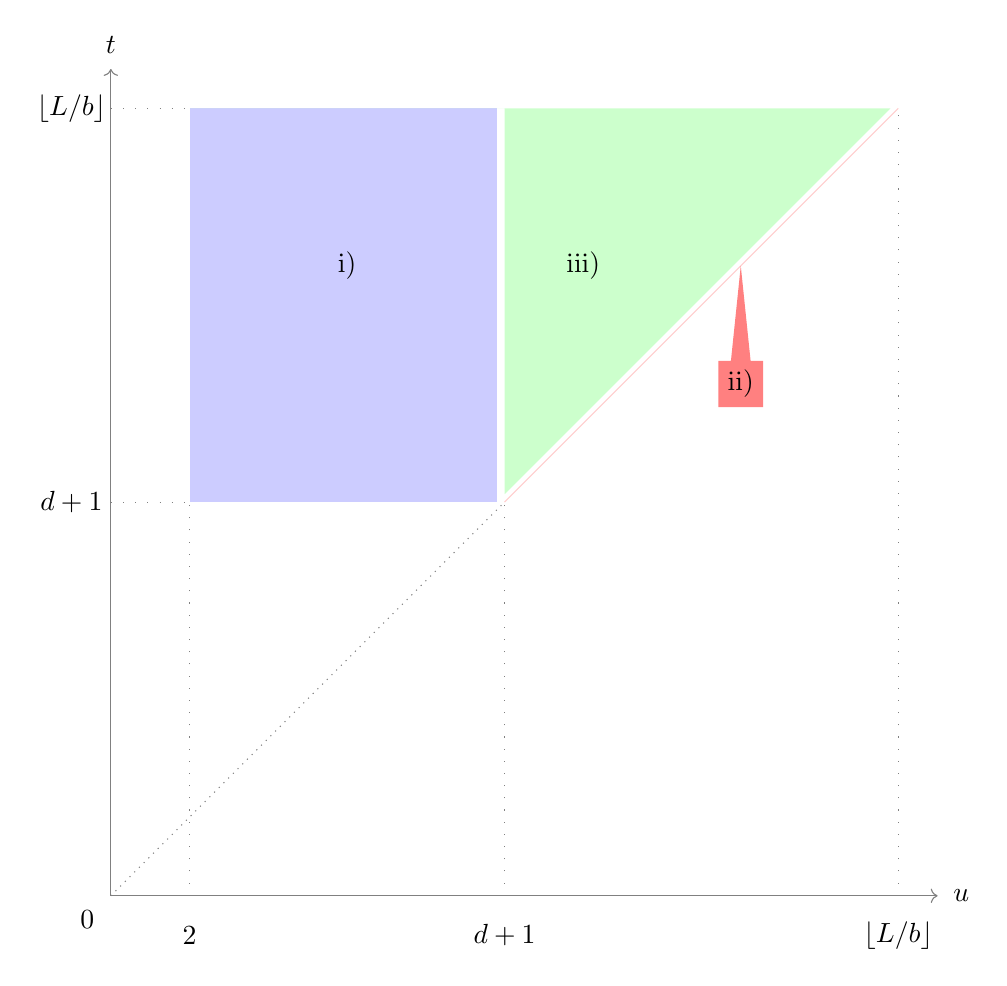
\begin{tikzpicture}[note/.style={rectangle callout, fill=#1}]
	\fill[blue!20] ( 1, 5) -- (4.9, 5) -- (4.9, 10) -- ( 1, 10);
	\fill[green!20] ( 5, 10) -- (5, 5.1) -- (9.9, 10) -- ( 1, 10);
	\draw[red!20] ( 5, 5) -- (10, 10);
	\draw[->,gray] ( 0, 0) -- (10.5, 0);
	\draw[->,gray] ( 0, 0) -- (0, 10.5);
	\draw[gray,loosely dotted] ( 1, 0) -- (1, 5);
	\draw[gray,loosely dotted] ( 10, 0) -- (10, 10);
	\draw[gray,loosely dotted] (  5, 0) -- (5, 5);
	\draw[gray,loosely dotted] (  0, 5) -- ( 1, 5);
	\draw[gray,loosely dotted] (  0,10) -- ( 1,10);
	\draw[gray,dotted] ( 0, 0) -- (5, 5);
	\draw ( -0.3, -0.3) node {$0$} ;
	\draw (10.8, 0) node {$u$} ;
	\draw (0, 10.8) node {$t$} ;
	\draw ( 1, -0.5) node {2} ;
	\draw ( 5, -0.5) node {$d+1$} ;
	\draw (10, -0.5) node {$\lfloor L/b \rfloor$} ;
	\draw ( -0.5, 5) node {$d+1$} ;
	\draw ( -0.5, 10) node {$\lfloor L/b \rfloor$} ;
	\draw ( 3, 8) node {i)} ;
	\draw ( 6, 8) node {iii)} ;
	\node [note=red!50, callout absolute pointer={(8,8)}] at (8,6.5) {ii)};
\end{tikzpicture}

\caption{Parameters $u, t$, where nested summation must be taken}\label{fig:param634}

\end{figure}

$t$-dependency of $F(z, t, u)$ must be considered when $u = t$.
From the above, the parameters domain where summation must be taken can be divided into the following three groups:

\begin{enumerate}[i)]
	%%%%%
	%%%%% i)
	%%%%%
	\item 
	\begin{align}
	\begin{cases}
		2 \leq u < d + 1 & \\
		d + 1 \leq t \leq \lfloor L / b \rfloor & 
	\end{cases}
	\label{eq:zone1_634}
	\end{align}
	%%%%%
	%%%%% ii)
	%%%%%
	\item 
	\begin{align}
	\begin{cases}
		(u, t) = (\tau, \tau) & \\
		d + 1 \leq \tau \leq \lfloor L / b \rfloor & 
	\end{cases}
	\label{eq:zone2_634}
	\end{align}
	%%%%%
	%%%%% iii)
	%%%%%
	\item 
	\begin{align}
	\begin{cases}
		d + 1 \leq u < t & \\
		d + 1 < t \leq \lfloor L / b \rfloor & 
	\end{cases}
	\label{eq:zone3_634}
	\end{align}
\end{enumerate}

For groups i) and iii), the summation with respect to $t$ can be taken first.
By using the relation $\nu = \lfloor L / b \rfloor - d$, Eq.(\ref{eq:rewGin634}) can be rewritten to as follows:
\begin{align}
G(z) =
& \sum_{u = 2}^{d} \log_{2}(u) z^{2} (1-z)^{u-1} \nonumber \\
& + \frac{1}{\nu} \sum_{u = d + 1}^{\lfloor L / b \rfloor} \log_{2}(u) z (1-z)^{u-1} \nonumber \\
& + \frac{1}{\nu} \sum_{u = d + 1}^{\lfloor L / b \rfloor - 1} (\lfloor L / b \rfloor - u) \log_{2}(u) z^{2} (1-z)^{u-1}
\label{eq:rewGin634performance}
\end{align}
With this expression, the computational complexity can be decreased from $\mathcal{O}(\nu^2)$ to $\mathcal{O}(\nu)$.

\subsection{Notes for t-Tuple estimate, LRS estimate, MultiMMC Prediction and LZ78Y prediction estimate}
In the following groups of entropy estimate, we have to handle $t$-tuples (pairs, triples, etc.)
\begin{enumerate}[a)]
	%%%%%
	%%%%% a)
	%%%%%
	\item t-Tuple estimate (NIST SP 800-90B 6.3.5)
	%%%%%
	%%%%% b)
	%%%%%
	\item Longest Repeated Substring (LRS) estimate (NIST SP 800-90B 6.3.6)
	%%%%%
	%%%%% c)
	%%%%%
	\item Multi Most Common in Window Prediction estimate (NIST SP 800-90B 6.3.7)
	%%%%%
	%%%%% d)
	%%%%%
	\item The MultiMMC Prediction estimate (NIST SP 800-90B 6.3.9)
	%%%%%
	%%%%% e)
	%%%%%
	\item The LZ78Y Prediction estimate (NIST SP 800-90B 6.3.10)
\end{enumerate}
In order to express $t$-tuples, bitset or multiprecision integer is used without using array.

\subsection{Notes for Multi Most Common in Window prediction estimate}
In step 3-a-i of 6.3.7 of NIST SP 800-90B, it is required to compute the mode in the previous window of $w_{j}$ before $s_{i}$. 
As the order of $w_{j}$ is 1000, the computational complexity is estimated to be about $\mathcal{O}(1000n)$, and expected to be time-consuming. 
We attempt to reduce time-complexity by preparing histograms of certain lengths in advance, and in step 3-a-i, we use the histograms that fit within the target window, and compute the unavailable parts on-demand basis.

%%%%%%%%%%%%%%%%%%%%%%%%%%%%%%%%%%%%%%%%%%%%%%%%%%%%%%%%%%%%%%%%%%%%%%%%%%%%%%%
%%%%%
%%%%% Bibliography
%%%%%
%%%%%%%%%%%%%%%%%%%%%%%%%%%%%%%%%%%%%%%%%%%%%%%%%%%%%%%%%%%%%%%%%%%%%%%%%%%%%%%
\setcounter{section}{2}
\begin{thebibliography}{99}
\addcontentsline{toc}{section}{References}
% 1
\bibitem{SP80090B}
Meltem S\"{o}nmez Turan,
Elaine Barker,
John Kelsey,
Kerry A. McKay,
Mary L. Baish,
Mike Boyle
\textit{Recommendation for the Entropy Sources Used for Random Bit Generation},
NIST Special Publication 800-90B, Jan. 2018
% 2
\bibitem{MathHandbook}
Franck W. J. Oliver,
Daniel W. Lozier,
Ronald F. Boisvert,
Charles W. Clark,
\textit{NIST Handbook of Mathematical Functions},
National Institute of Standards and Technology, 2010
% 6
\bibitem{CorrectionsSP80090B}
G. Sakurai, \textit{Proposed list of corrections for NIST SP 800-90B 6.3 Estimators}, Dec. 2022
\url{https://github.com/g-g-sakura/AnotherEntropyEstimationTool/blob/main/documentation/ProposedListOfCorrections_SP800-90B.pdf}
% 7
\bibitem{AIS31draft2022}
M. Peter and W. Schindler,
\textit{A Proposal for Functionality Classes for Random Number Generators}
Version 2.35 - DRAFT,
September 2, 2022.
\url{https://www.bsi.bund.de/SharedDocs/Downloads/EN/BSI/Certification/Interpretations/AIS_31_Functionality_classes_for_random_number_generators_e.pdf?__blob=publicationFile&v=7}
\end{thebibliography}

\end{document}
